\documentclass[11pt,a4paper]{article}
\usepackage[margin=2cm]{geometry}
\usepackage{lmodern}
\usepackage[T1]{fontenc}
\usepackage{amsmath,amssymb}
\usepackage{booktabs,array}
\usepackage{enumitem}
\usepackage{xcolor}
\usepackage[most]{tcolorbox}
\usepackage{titlesec}
\usepackage{graphicx}
\usepackage{float}
\usepackage{needspace}
\usepackage[font=small,labelfont={bf,color=headblue},skip=4pt]{caption}
\usepackage[colorlinks=true,linkcolor=black,urlcolor=blue!50!black]{hyperref}

\definecolor{headblue}{RGB}{38,70,120}
\titleformat{\section}{\Large\bfseries\color{headblue}}{\thesection}{0.8em}{}[{\color{black}\titlerule}]
\titleformat{\subsection}{\large\bfseries\color{headblue}}{\thesubsection}{0.8em}{}
\titlespacing*{\section}{0pt}{12pt}{6pt}
\titlespacing*{\subsection}{0pt}{8pt}{3pt}
\setlength{\parindent}{0pt}
\setlength{\parskip}{5pt}
\setlist{itemsep=2pt,topsep=2pt}
\setlength{\emergencystretch}{3em}
\renewcommand{\arraystretch}{1.12}
\newtcolorbox{keybox}{colback=blue!3,colframe=headblue!60,boxrule=0.5pt,arc=2mm,left=2mm,right=2mm,top=1mm,bottom=1mm}
\newcommand{\pct}{\,\%}
% keep a section heading together with the start of its text
\newcommand{\sect}[1]{\section{#1}}

% headline numbers, generated by make_figures.py from the run
% generated by make_figures.py
\newcommand{\NInst}{560}
\newcommand{\NOpt}{256}
\newcommand{\NTL}{223}
\newcommand{\NNone}{30}
\newcommand{\NInf}{51}
\newcommand{\NValid}{479}
\newcommand{\GapMed}{4.2}
\newcommand{\GapMax}{26.9}
\newcommand{\NEV}{24250}
\newcommand{\NFree}{20584}
\newcommand{\NStranded}{3666}
\newcommand{\TimeLimit}{300}
\newcommand{\Workers}{8}
\newcommand{\Threads}{4}
\newcommand{\InfSame}{the same}
\newcommand{\VanAll}{7.0}
\newcommand{\VanLowOpt}{0.0}
\newcommand{\VanSixSeven}{7.7}
\newcommand{\VanSevenEight}{16.6}
\newcommand{\VanEightNine}{35.5}
\newcommand{\VanNineTen}{31.4}
\newcommand{\VanTopAll}{31.7}
\newcommand{\VanBotAll}{0.9}
\newcommand{\LowVanOpt}{0}
\newcommand{\LowVanTL}{74}
\newcommand{\ThetaVan}{0.74}
\newcommand{\ThetaFCS}{0.48}
\newcommand{\PressLow}{0.14}
\newcommand{\PressHigh}{0.41}
\newcommand{\QLow}{0.03}
\newcommand{\QueuingLow}{0.4}
\newcommand{\TopLow}{43.3}
\newcommand{\LowQLow}{0.05}
\newcommand{\TopQLow}{0.00}
\newcommand{\QMid}{0.08}
\newcommand{\QueuingMid}{1.3}
\newcommand{\TopMid}{27.8}
\newcommand{\LowQMid}{0.13}
\newcommand{\TopQMid}{0.00}
\newcommand{\QHigh}{4.08}
\newcommand{\QueuingHigh}{20.9}
\newcommand{\TopHigh}{21.1}
\newcommand{\LowQHigh}{8.38}
\newcommand{\TopQHigh}{0.62}
\newcommand{\QShareBottom}{72.8}
\newcommand{\UShareBottom}{35.6}
\newcommand{\QShareTop}{1.1}
\newcommand{\UShareTop}{7.2}
\newcommand{\DriveBot}{2.69}
\newcommand{\DriveTop}{1.78}
\newcommand{\TopShort}{27.3}
\newcommand{\PressShort}{0.53}
\newcommand{\TopLong}{35.8}
\newcommand{\PressLong}{0.45}
\newcommand{\PaidBot}{302}
\newcommand{\PaidTop}{369}
\newcommand{\FeltBot}{585}
\newcommand{\FeltTop}{694}
\newcommand{\MoneyBot}{410}
\newcommand{\MoneyTop}{230}
\newcommand{\TimeBot}{175}
\newcommand{\TimeTop}{464}
\newcommand{\ZOne}{0.8}
\newcommand{\ZTwo}{2.3}
\newcommand{\ZThree}{6.9}
\newcommand{\ZFour}{19.6}
\newcommand{\ZFive}{35.3}
\newcommand{\ZSix}{35.1}
\newcommand{\ZOperator}{28.8}
\newcommand{\ZCustomer}{71.2}
\newcommand{\VanWaitBot}{142}
\newcommand{\VanWaitTop}{9}
\newcommand{\AME}{4.0}
\newcommand{\AMEHigh}{2.5}
\newcommand{\AMENotHigh}{4.8}
\newcommand{\LogitAcc}{93.1}
\newcommand{\LogitN}{20584}


\begin{document}

\begin{center}
{\LARGE\bfseries\color{headblue} Income and the choice of charger}\\[6pt]
{\large Results of formulation 3 on the EV-Solomon dataset}\\[4pt]
{\normalsize CP 320 Operations Research for Mobility, course project}\\[2pt]
{\normalsize Yakshith Maddineni (SR 26080) \quad\textperiodcentered\quad Kartikeya Gaur (SR 26371)}\\[2pt]
{\normalsize 22 November 2026}
\end{center}

\begin{keybox}
{\color{headblue}\textbf{Key findings}}
\begin{enumerate}[leftmargin=1.4em]
  \item \textbf{Income decides who gets a van.} In the proven-optimal plans no customer with income below $\theta=0.4$ is served by a van. The van share then rises to \VanSixSeven\pct{} ($\theta$ 0.6--0.7), \VanSevenEight\pct{} (0.7--0.8) and \VanEightNine\pct{} (0.8--0.9).
  \item \textbf{Low-income customers absorb the queues.} The poorest 40\pct{} of station users do \QShareBottom\pct{} of all queueing; the richest 20\pct{} do \QShareTop\pct{}. Low-income customers also drive farther to their station (\DriveBot{} km against \DriveTop{} km).
  \item \textbf{At peak demand, income buys a place at the station rather than a van.} When demand is high, vans are already busy. The richest customers' van share falls from \TopLow\pct{} to \TopHigh\pct{}, but they still queue only \TopQHigh{} min on average, against \LowQHigh{} min for the poorest 40\pct.
  \item \textbf{Time and congestion, not the horizon itself.} High-income customers get vans more often in the long-horizon families (\TopLong\pct{} against \TopShort\pct{}). Once demand pressure is accounted for, the horizon has no separate effect.
  \item \textbf{The solver results are sound.} All \NValid{} plans pass an independent check. The \NInf{} infeasible instances are \InfSame{} as in the main-formulation run, so they come from the data, not from the income model.
\end{enumerate}
\end{keybox}

%=====================================================================
\sect{What was run}

Formulation 3 gives every EV an income index $\theta_i\in[0,1]$ (0 = lowest, 1 = highest income). Income sets three sensitivities of the customer: the money sensitivity $\mu(\theta)$ (falls with income), the values of time $c^{a}(\theta)$ for driving, queueing, charging at a station and the van service (rise with income), and the queue tolerance $W(\theta)$ (falls with income). The model minimises the operator's cost plus the cost each customer perceives. Who is served at a fixed station (FCS) and who by a mobile van (MCS) is therefore an outcome, not an input.

\textbf{Run.} The 56 Solomon files of EV-Solomon, each for its first $n=10,20,\dots,100$ EVs: \NInst{} instances. Every instance was given to Gurobi 13 with the complete model, a time limit of \TimeLimit\,s and a greedy plan as warm start, \Workers{} instances at a time with \Threads{} threads each on the lab server. Table~\ref{tab:params} lists the income parameters. They are placeholder values; the formulation itself only fixes their directions. All figures and tables below are made by \texttt{make\_figures.py} in this folder from \texttt{../results.csv} and \texttt{../analysis/ev\_level.csv}.

\textbf{Terms used below.}
\begin{itemize}
  \item \emph{Free-choice EV}: an EV with at least one station in range. The \NStranded{} stranded EVs (of \NEV) must take a van whatever their income, so all shares below are over the \NFree{} free-choice EVs.
  \item \emph{Income band}: $\theta$ in 0.0--0.2, 0.2--0.4, 0.4--0.6, 0.6--0.8, 0.8--1.0.
  \item \emph{Demand pressure} of a request: the number of requests released during the preceding mean charging time, divided by the number of chargers (24 guns + 5 vans). It uses only the data, not the plan. The pooled terciles give \emph{low} ($\le\PressLow$), \emph{medium} and \emph{high} ($>\PressHigh$) pressure; this replaces a peak/off-peak label.
  \item \emph{Optimal plan}: Gurobi proved optimality. A \emph{time-limit plan} is valid but not proven optimal.
\end{itemize}

\begin{table}[H]
\centering\small
\caption{Income parameters of the run (straight lines between $\theta=0$ and $\theta=1$).}
\label{tab:params}
\begin{tabular}{@{}llrr@{}}
\toprule
parameter & unit & at $\theta=0$ & at $\theta=1$ \\
\midrule
income $\theta_i$ & -- & Beta(2, 2) &  \\
money sensitivity $\mu$ & Rs/Rs & 1.5 & 0.5 \\
value of time $c^{\mathrm{D}}$ (driving to an FCS) & Rs/min & 1.5 & 15 \\
value of time $c^{\mathrm{Q}}$ (queueing at an FCS) & Rs/min & 2.5 & 25 \\
value of time $c^{\mathrm{C}}$ (charging at an FCS) & Rs/min & 1 & 10 \\
value of time $c^{\mathrm{V}}$ (van wait + van charging) & Rs/min & 0.5 & 5 \\
queue tolerance $W$ & min & 60 & 15 \\
tariff $p^{\mathrm F}$ / $p^{\mathrm M}$ & Rs/kWh & 15 & 25 \\
\bottomrule
\end{tabular}

\end{table}

%=====================================================================
\sect{Solver outcome}

\begin{itemize}
  \item \textbf{\NOpt{}} instances were solved to optimality and \textbf{\NTL{}} ended at the time limit with a plan (median gap \GapMed\pct, largest \GapMax\pct). All \NValid{} plans pass the independent checker, which tests every constraint and recomputes $Z$.
  \item \textbf{\NInf{}} instances are infeasible. They are \InfSame{} 51 instances that were infeasible in the main-formulation run of October: Solomon's deadline $T$ is too short to charge some EVs in time, with or without income.
  \item \textbf{\NNone{}} instances (R1 and RC1 with $n\ge70$, and C204 with $n=100$) ended without any plan. They are \emph{unsolved}, not proven infeasible: the greedy start plan fails once the queue limits $W_i$ apply, and Gurobi found no feasible plan within \TimeLimit\,s.
\end{itemize}

\begin{figure}[H]
\centering
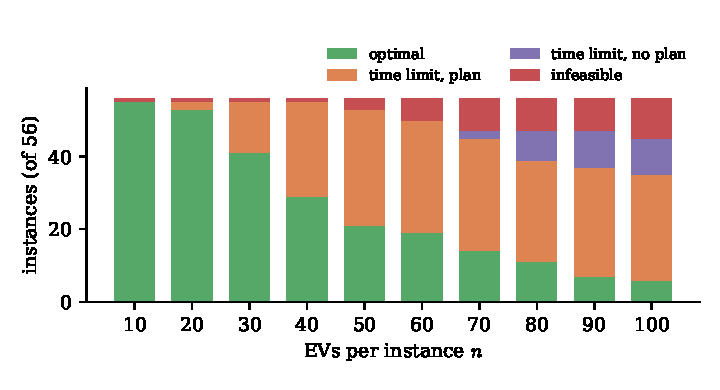
\includegraphics[width=0.66\textwidth]{figures/solver_outcome.pdf}
\caption{How the 56 instances of each size ended.}
\label{fig:solver}
\end{figure}

\begin{table}[H]
\centering\small
\caption{Solver outcome per instance size. The gap is that of the time-limit plans.}
\label{tab:solver}
\begin{tabular}{@{}rrrrrrrr@{}}
\toprule
$n$ & instances & optimal & \shortstack[r]{time limit\\with plan} & \shortstack[r]{time limit\\no plan} & infeasible & \shortstack[r]{median\\gap (\%)} & \shortstack[r]{mean\\time (s)} \\
\midrule
10 & 56 & 55 & 0 & 0 & 1 & -- & 0 \\
20 & 56 & 53 & 2 & 0 & 1 & 1.02 & 23 \\
30 & 56 & 41 & 14 & 0 & 1 & 1.88 & 96 \\
40 & 56 & 29 & 26 & 0 & 1 & 3.66 & 154 \\
50 & 56 & 21 & 32 & 0 & 3 & 5.91 & 182 \\
60 & 56 & 19 & 31 & 0 & 6 & 7.54 & 186 \\
70 & 56 & 14 & 31 & 2 & 9 & 6.98 & 191 \\
80 & 56 & 11 & 28 & 8 & 9 & 3.53 & 218 \\
90 & 56 & 7 & 30 & 10 & 9 & 2.13 & 236 \\
100 & 56 & 6 & 29 & 10 & 11 & 2.76 & 221 \\
\midrule
all & 560 & 256 & 223 & 30 & 51 & 4.22 & 151 \\
\bottomrule
\end{tabular}

\end{table}

%=====================================================================
\sect{Income decides who gets a van}
\label{sec:van}

\begin{itemize}
  \item Overall \VanAll\pct{} of the free-choice EVs get a van. Van users have a mean income of \ThetaVan, station users \ThetaFCS.
  \item In the optimal plans the share is exactly \VanLowOpt\pct{} below $\theta=0.4$, small up to $\theta=0.6$, and then rises steeply: \VanSixSeven\pct, \VanSevenEight\pct, \VanEightNine\pct{} (Figure~\ref{fig:van}). This is the income threshold $\theta^{*}_i$ of Section 4.1 of the formulation: below it the van premium weighs more than the time saved, above it the time saved wins.
  \item The share stops rising at the top (\VanNineTen\pct{} for 0.9--1.0): the vans are full. With 5 vans of 6 EVs each and the stranded EVs taking their seats first, not every high-income customer can get one.
  \item \textbf{Low-income van users are artefacts.} The \LowVanTL{} free-choice EVs with $\theta<0.4$ that got a van all come from time-limit plans (\LowVanOpt{} in optimal plans). They wait \VanWaitBot{} min for the van on average, against \VanWaitTop{} min for the richest band: Gurobi had not finished improving those plans.
\end{itemize}

\begin{figure}[H]
\centering
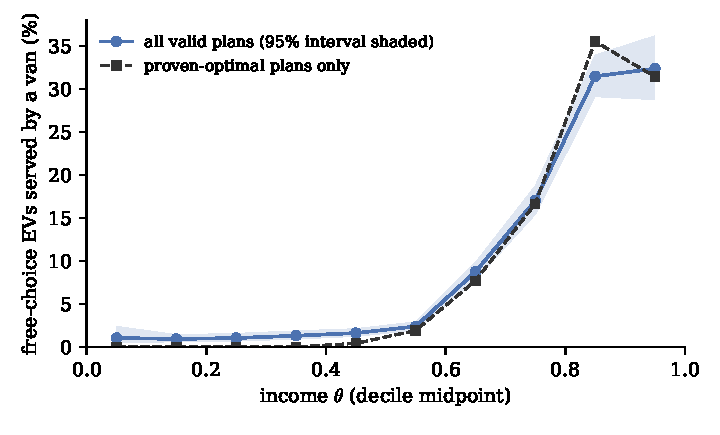
\includegraphics[width=0.66\textwidth]{figures/van_by_income.pdf}
\caption{Share of free-choice EVs served by a van, by income decile.}
\label{fig:van}
\end{figure}

\begin{table}[H]
\centering\small
\caption{Van share by income decile; interval = 95\pct{} Wilson interval of the share over all valid plans.}
\label{tab:deciles}
\begin{tabular}{@{}lrrrrr@{}}
\toprule
income $\theta$ & EVs & \shortstack[r]{by van\\(\%)} & \shortstack[r]{95\,\%\\interval} & \shortstack[r]{EVs\\(optimal plans)} & \shortstack[r]{by van (\%)\\(optimal plans)} \\
\midrule
0.0--0.1 & 485 & 1.0 & [0.4, 2.4] & 182 & 0.0 \\
0.1--0.2 & 2182 & 0.9 & [0.6, 1.4] & 867 & 0.0 \\
0.2--0.3 & 2050 & 1.0 & [0.7, 1.6] & 846 & 0.0 \\
0.3--0.4 & 2168 & 1.3 & [0.9, 1.9] & 692 & 0.0 \\
0.4--0.5 & 3061 & 1.6 & [1.2, 2.1] & 997 & 0.4 \\
0.5--0.6 & 3754 & 2.4 & [1.9, 2.9] & 1371 & 1.9 \\
0.6--0.7 & 2929 & 8.7 & [7.8, 9.8] & 1262 & 7.7 \\
0.7--0.8 & 1941 & 17.0 & [15.4, 18.7] & 811 & 16.6 \\
0.8--0.9 & 1408 & 31.5 & [29.1, 33.9] & 566 & 35.5 \\
0.9--1.0 & 606 & 32.3 & [28.7, 36.2] & 226 & 31.4 \\
\bottomrule
\end{tabular}

\end{table}

%=====================================================================
\sect{Who waits: queues and driving}

\begin{itemize}
  \item The poorest 40\pct{} are \UShareBottom\pct{} of the station users but do \QShareBottom\pct{} of all queueing. The richest 20\pct{} are \UShareTop\pct{} of the users and do \QShareTop\pct{} (Figure~\ref{fig:queues}).
  \item Nobody is pushed to the limit of their patience: in every band the longest queue stays below the largest $W_i$ of the band (Table~\ref{tab:queues}). The queues follow from the cost weights ($c^{\mathrm Q}$ rises with income), not only from the hard limit.
  \item Low-income station users drive farther (\DriveBot{} km against \DriveTop{} km), although they feel the driving cost most ($\mu$ is largest). The free guns at the nearest stations go to the customers whose time is worth most; the others drive on or wait.
\end{itemize}

\begin{figure}[H]
\centering
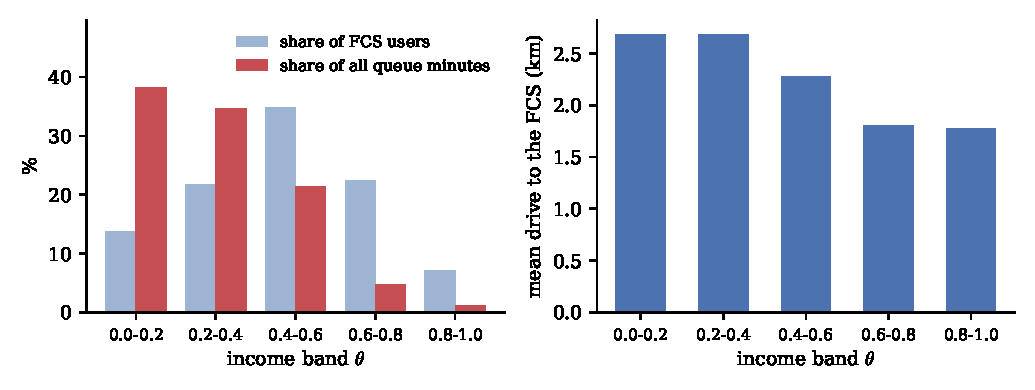
\includegraphics[width=\textwidth]{figures/queues_drive.pdf}
\caption{Left: share of station users and share of all queue minutes by income band. Right: mean distance driven to the station.}
\label{fig:queues}
\end{figure}

\begin{table}[H]
\centering\footnotesize
\caption{Station users by income band.}
\label{tab:queues}
\begin{tabular}{@{}lrrrrrrrr@{}}
\toprule
income $\theta$ & \shortstack[r]{FCS\\users} & \shortstack[r]{share of\\users (\%)} & \shortstack[r]{share of queue\\minutes (\%)} & \shortstack[r]{queueing\\(\%)} & \shortstack[r]{mean queue\\(min)} & \shortstack[r]{longest\\queue (min)} & \shortstack[r]{largest\\$W_i$ (min)} & \shortstack[r]{drive to\\FCS (km)} \\
\midrule
0.0--0.2 & 2642 & 13.8 & 38.2 & 13.6 & 3.79 & 55.8 & 59.3 & 2.69 \\
0.2--0.4 & 4169 & 21.8 & 34.6 & 10.9 & 2.18 & 48.8 & 50.7 & 2.69 \\
0.4--0.6 & 6677 & 34.9 & 21.3 & 6.5 & 0.84 & 40.3 & 42.0 & 2.27 \\
0.6--0.8 & 4284 & 22.4 & 4.7 & 2.9 & 0.29 & 30.8 & 33.0 & 1.80 \\
0.8--1.0 & 1375 & 7.2 & 1.1 & 3.1 & 0.22 & 20.8 & 23.9 & 1.78 \\
\bottomrule
\end{tabular}

\end{table}

%=====================================================================
\sect{Peak and off-peak: demand pressure}

\begin{itemize}
  \item Demand pressure separates calm and busy periods well. Queues are almost absent at low and medium pressure (\QLow{} and \QMid{} min on average). At high pressure \QueuingHigh\pct{} of station users queue, \QHigh{} min on average.
  \item \textbf{At high pressure, fewer high-income customers get a van}: \TopLow\pct{} at low pressure, \TopMid\pct{} at medium and \TopHigh\pct{} at high pressure (Figure~\ref{fig:pressure}). The vans are already committed to stranded EVs, and there is little spare van time.
  \item \textbf{Instead, income buys priority at the station.} At high pressure the richest band queues \TopQHigh{} min on average, the poorest 40\pct{} \LowQHigh{} min.
  \item Low-income customers stay at the stations even at high pressure. The few low-income van users in the high-pressure row of Table~\ref{tab:pressure} all come from time-limit plans.
\end{itemize}

\begin{figure}[H]
\centering
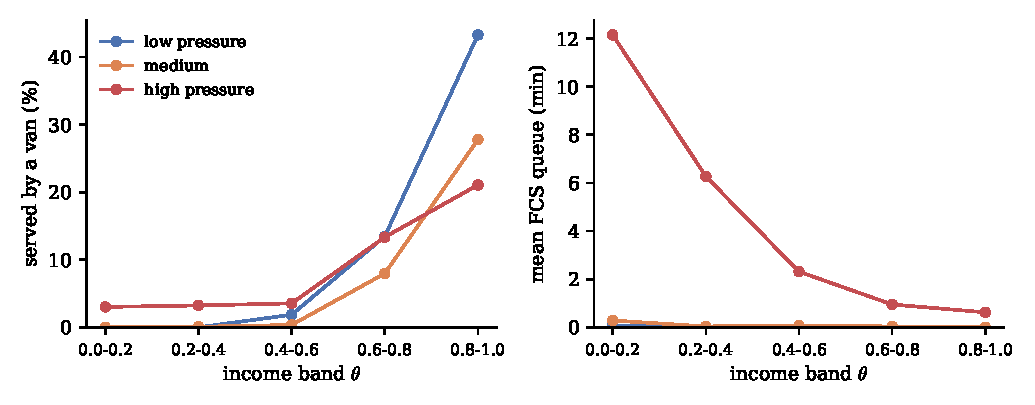
\includegraphics[width=\textwidth]{figures/pressure.pdf}
\caption{Van share (left) and mean station queue (right) by income band, for low, medium and high demand pressure.}
\label{fig:pressure}
\end{figure}

\begin{table}[H]
\centering\footnotesize
\caption{Free-choice EVs by demand pressure.}
\label{tab:pressure}
\begin{tabular}{@{}lrrrrrrrrr@{}}
\toprule
\shortstack[l]{demand\\pressure} & EVs & \shortstack[r]{queueing\\(\%)} & \shortstack[r]{mean queue\\(min)} & \shortstack[r]{by van\\(\%)} & \shortstack[r]{by van\\$\theta$ 0.0--0.2} & \shortstack[r]{by van\\$\theta$ 0.2--0.4} & \shortstack[r]{by van\\$\theta$ 0.4--0.6} & \shortstack[r]{by van\\$\theta$ 0.6--0.8} & \shortstack[r]{by van\\$\theta$ 0.8--1.0} \\
\midrule
low & 8168 & 0.4 & 0.03 & 8.3 & 0.0 & 0.0 & 1.9 & 13.5 & 43.3 \\
medium & 5663 & 1.3 & 0.08 & 5.0 & 0.0 & 0.1 & 0.4 & 8.0 & 27.8 \\
high & 6753 & 20.9 & 4.08 & 7.0 & 3.0 & 3.2 & 3.5 & 13.4 & 21.1 \\
\bottomrule
\end{tabular}

\end{table}

%=====================================================================
\sect{Short and long planning horizons}

\begin{itemize}
  \item High-income customers get a van more often when the horizon is long: \TopLong\pct{} against \TopShort\pct{} in the top band (Figure~\ref{fig:horizon}). The gap is largest for R (R2 against R1) and RC; for the clustered layout C the two horizons are close (Table~\ref{tab:families}).
  \item The short-horizon families are also more congested (mean demand pressure \PressShort{} against \PressLong). In the regression of Section~\ref{sec:logit}, which includes demand pressure, the horizon itself has no effect. The horizon matters because it sets how busy the chargers and vans are.
\end{itemize}

\begin{figure}[H]
\centering
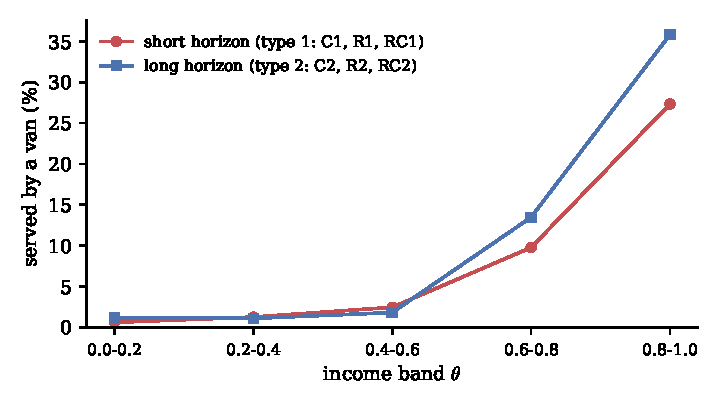
\includegraphics[width=0.66\textwidth]{figures/horizon.pdf}
\caption{Van share by income band in the short-horizon (type 1) and long-horizon (type 2) families.}
\label{fig:horizon}
\end{figure}

\begin{table}[H]
\centering\footnotesize
\caption{Van share by family and income band.}
\label{tab:families}
\begin{tabular}{@{}llrrrrrrrr@{}}
\toprule
family & horizon & EVs & \shortstack[r]{mean\\pressure} & \shortstack[r]{by van\\(\%)} & \shortstack[r]{by van\\$\theta$ 0.0--0.2} & \shortstack[r]{by van\\$\theta$ 0.2--0.4} & \shortstack[r]{by van\\$\theta$ 0.4--0.6} & \shortstack[r]{by van\\$\theta$ 0.6--0.8} & \shortstack[r]{by van\\$\theta$ 0.8--1.0} \\
\midrule
C1 & short & 4104 & 0.38 & 6.9 & 0.9 & 1.5 & 0.4 & 6.2 & 37.0 \\
C2 & long & 3771 & 0.29 & 8.9 & 1.4 & 0.8 & 3.9 & 13.5 & 36.8 \\
R1 & short & 2493 & 0.69 & 5.6 & 0.3 & 0.7 & 2.5 & 13.7 & 17.5 \\
R2 & long & 5082 & 0.56 & 5.9 & 1.5 & 1.4 & 1.0 & 11.2 & 49.2 \\
RC1 & short & 1454 & 0.69 & 7.8 & 0.4 & 1.8 & 6.5 & 20.1 & 16.2 \\
RC2 & long & 3680 & 0.46 & 7.2 & 0.6 & 0.9 & 1.4 & 17.4 & 27.2 \\
\bottomrule
\end{tabular}

\end{table}

%=====================================================================
\sect{What customers pay and what they feel}

\begin{itemize}
  \item Customers in the lowest band pay \PaidBot{} Rs on average and perceive \FeltBot{} Rs (\MoneyBot{} Rs money, \TimeBot{} Rs time). In the top band they pay more, \PaidTop{} Rs, because more of them use the dearer van, and perceive \FeltTop{} Rs (\MoneyTop{} Rs money, \TimeTop{} Rs time). For the poor the money dominates; for the rich, time does (Figure~\ref{fig:costs}).
  \item Over all valid plans the customers' perceived cost is \ZCustomer\pct{} of the objective (tariff \ZFive\pct, time \ZSix\pct, driving \ZOne\pct) and the operator's cost \ZOperator\pct{} (energy \ZFour\pct, van dispatch \ZThree\pct, van driving \ZTwo\pct).
\end{itemize}

\begin{figure}[H]
\centering
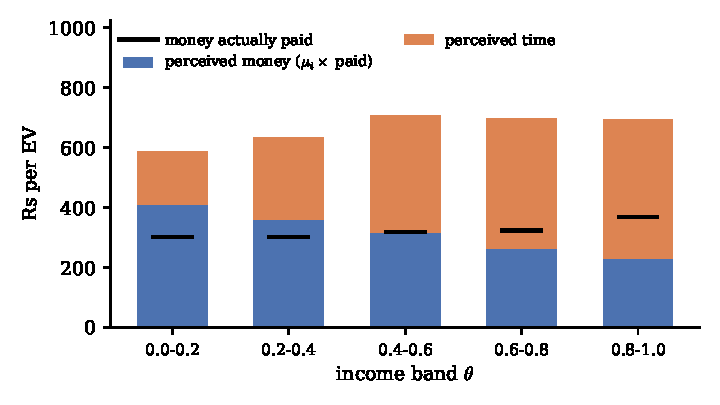
\includegraphics[width=0.66\textwidth]{figures/costs.pdf}
\caption{Mean money paid and mean perceived cost (money weighted by $\mu_i$, plus time) per EV by income band.}
\label{fig:costs}
\end{figure}

\begin{table}[H]
\centering\small
\caption{Money and perceived cost per free-choice EV by income band.}
\label{tab:costs}
\begin{tabular}{@{}lrrrrr@{}}
\toprule
income $\theta$ & \shortstack[r]{paid\\(Rs)} & \shortstack[r]{perceived\\money (Rs)} & \shortstack[r]{perceived\\time (Rs)} & \shortstack[r]{perceived\\total (Rs)} & \shortstack[r]{request to\\charged (min)} \\
\midrule
0.0--0.2 & 302 & 410 & 175 & 585 & 68.1 \\
0.2--0.4 & 301 & 359 & 273 & 633 & 66.0 \\
0.4--0.6 & 318 & 316 & 390 & 706 & 65.6 \\
0.6--0.8 & 323 & 264 & 432 & 696 & 60.1 \\
0.8--1.0 & 369 & 230 & 464 & 694 & 57.5 \\
\bottomrule
\end{tabular}

\end{table}

%=====================================================================
\sect{Logistic regression}
\label{sec:logit}

To see each factor with the others held fixed, we fit a logistic regression of ``served by a van'' over the \LogitN{} free-choice EVs (Table~\ref{tab:logit}).

\begin{itemize}
  \item Income has a strong positive effect. On average, $+0.1$ in $\theta$ raises the probability of a van by \AME{} percentage points: \AMENotHigh{} points at low or medium pressure and \AMEHigh{} at high pressure (the negative $\theta\times$ high-pressure term).
  \item An EV far from its nearest reachable station is more likely to get a van. An EV with a larger energy demand is less likely, because the van premium and the van's battery use grow with the energy.
  \item The long horizon has no effect of its own once demand pressure is included. The model classifies \LogitAcc\pct{} of the EVs correctly. The regression uses all valid plans, so the time-limit artefacts of Section~\ref{sec:van} are included.
\end{itemize}

\begin{table}[H]
\centering\small
\caption{Logistic regression of $P(\text{served by a van})$.}
\label{tab:logit}
\begin{tabular}{@{}lrrrr@{}}
\toprule
term & coefficient & std.\ error & $z$ & $p$-value \\
\midrule
intercept & -9.036 & 0.256 & -35.2 & $<0.001$ \\
income $\theta$ & 9.806 & 0.289 & 33.9 & $<0.001$ \\
medium pressure & -0.851 & 0.085 & -10.0 & $<0.001$ \\
high pressure & 3.839 & 0.275 & 14.0 & $<0.001$ \\
$\theta\times$ high pressure & -5.715 & 0.381 & -15.0 & $<0.001$ \\
long horizon (type 2) & -0.030 & 0.066 & -0.5 & 0.649 \\
energy $E_i$ (per 10 kWh) & -0.250 & 0.056 & -4.5 & $<0.001$ \\
nearest reachable FCS (km) & 0.449 & 0.038 & 11.8 & $<0.001$ \\
\bottomrule
\end{tabular}

\end{table}

%=====================================================================
\sect{What to keep in mind}

\begin{itemize}
  \item \textbf{Where the threshold lies comes from the parameter values.} That income raises the chance of a van follows from the formulation; where the threshold lies (near $\theta=0.6$ here) and how steep the step is follow from the placeholder values in Table~\ref{tab:params}. Runs with other values of the van premium $p^{\mathrm M}-p^{\mathrm F}$, the slopes of $c^{a}(\theta)$ and the fleet size would show how the threshold moves.
  \item \textbf{Time-limit plans are not optimal.} They are valid, but they contain placements that a finished optimisation would remove, such as low-income van users with long waits.
  \item \textbf{\NNone{} instances have no plan}, so the largest congested R1 and RC1 instances are missing from the analysis. A better start plan or a longer time limit would fill them in.
  \item \textbf{Income is independent of location.} $\theta_i$ is drawn per EV without regard to where the EV is; richer and poorer neighbourhoods are not modelled.
\end{itemize}

\end{document}
